\RequirePackage{nag}
\documentclass[12pt,letterpaper]{article}
\usepackage{lipsum}
% \usepackage{fixltx2e}
% \usepackage{classicthesis}
\usepackage{polyglossia}
\usepackage[natbib=true, 
			style=numeric, %authoryear or numeric; comp == compact
			bibstyle=nature, 
			backend=biber,
			uniquelist=false, 
			sorting=none,
			uniquename=false]{biblatex}
\usepackage{booktabs}
\usepackage{relsize}
\usepackage{setspace}
\usepackage{lineno}
\usepackage{wrapfig}
\usepackage{sidecap}

\setdefaultlanguage{english}
\setmainfont[Mapping=tex-text, 
			 Numbers=OldStyle, 
			 % SizeFeatures={{Size=12}}
			 ]{Times}
\setsansfont[Mapping=tex-text, 
			 Numbers=OldStyle, 
			 % SizeFeatures={{Size=12}}
			 ]{Helvetica}
\setmonofont[Scale=0.8]{Monaco}
\setcounter{secnumdepth}{0}

\addbibresource{ELI.bib}

% Set the line spread (height). Be careful here, use too small rather than too
% large value. Also: double-spaced lines correspond to a value of ~1.3,
% depending on the font, NOT to 2.0
\setstretch{1.1} % 1.1 normally

\graphicspath{{figs/}}

%% Custom macros

\newcommand*\captitle[1]{\textbf{#1}}
\newcommand*\todo[1]{%
    \graffito{\textcolor{red}{TO\ DO: #1}}}

\newcommand*\gene[1]{\textit{#1}}
\newcommand*\ko[1]{\textit{#1\textsuperscript{\(-/-\)}}}
\newcommand*\protein[1]{#1}
\newcommand*\species[1]{\textit{#1}}


\title{\ruleline{Management Plan}}
\lhead{Zhian N. Kamvar, Ph. D.}
\rhead{Management Plan}

\begin{document}
\maketitle

% The plan is to be clearly articulated and include an organizational chart,
% administrative timeline, and a description of how the project will be governed,
% as well as a strategy to enhance coordination, collaboration, communication, and
% data sharing and reporting among members of the project team and stakeholder
% groups. The plan must also address how the project will be sustained beyond
% termination of an award. 

% The management plan must also include an advisory group of principal
% stakeholders, partners, and professionals to assess and evaluate the quality,
% expected measurable outcomes, and potential impacts for the proposed research,
% education and/or extension. Please include rationale for their role, and how
% they will function effectively to support the goals and objectives of the
% project. The plan must demonstrate how partners and stakeholders contribute to
% project assessment on an annual basis.

\section{Overview}

This project will be conducted by Dr. Zhian N. Kamvar at the University of Nebraska-Lincoln (UNL) in the department of Plant Pathology. 
Primary mentoring activities will be provided by Dr. Sydney E. Everhart, who is experienced in molecular techniques and evolutionary biology. 
The collaborating mentor, Dr. Jenny Dauer, who is experienced in evidence-based evaluation of scientific teaching and learning, will serve as mentor in educational activities.


\subsubsection*{Objective \#1: Development of Education Modules on Open and Reproducible Research}

The fellow will provide all materials including research, web infrastructure, data sets, and evaluation instruments. 
Drs. Dauer and Everhart will provide guidance based on monthly reports and quarterly reviews.

\subsubsection*{Objective \#2: Whole Genome Sequencing of 96 \textit{Sclerotinia sclerotiorum} isolates}

The fellow will pre-register the project design on the Open Science Framework (OSF, \url{https://osf.io}).
After receipt of isolates from China he fellow will grow and harvest mycelia from 96 isolates of \textit{S. sclerotiorum} for DNA extraction under the supervision of Dr. Sydney Everhart. 
Purified DNA will be sent to BGI, where sequencing will be performed by trained technicians. \
Sequences will be delivered to the fellow on BGI-hosted servers.

\subsubsection*{Objective \#3: Assessment of Local Adaptation to Climate}

The fellow will retrieve the sequences and archive them at OSF and copy them to UNL servers. 
All alignment scripts will be hosted on GitHub (\url{https://github.com}), linked to OSF. Dr. 
Everhart will provide guidance on progress based on monthly reports and quarterly reviews.

\subsubsection*{Objective \#4: Leading and Evaluating Special Topics Course}

The fellow will register the course, recruit participants, administer pre- and post- course evaluation instruments, and lead the course. 
Evaluation will be based on how well the course progress aligns with the learning objectives. 

\section{Administrative Timeline, Communication, and Assessment}

The project timeline is provided in figure \ref{fig:timeline}. 
The Fellow will submit monthly reports and have quarterly review meetings with both Dr. Everhart and Dr. Dauer. 
Any changes to the timeline must be approved by both Primary and Collaborative mentors. 

\begin{figure}[!htbp]
  \centering
  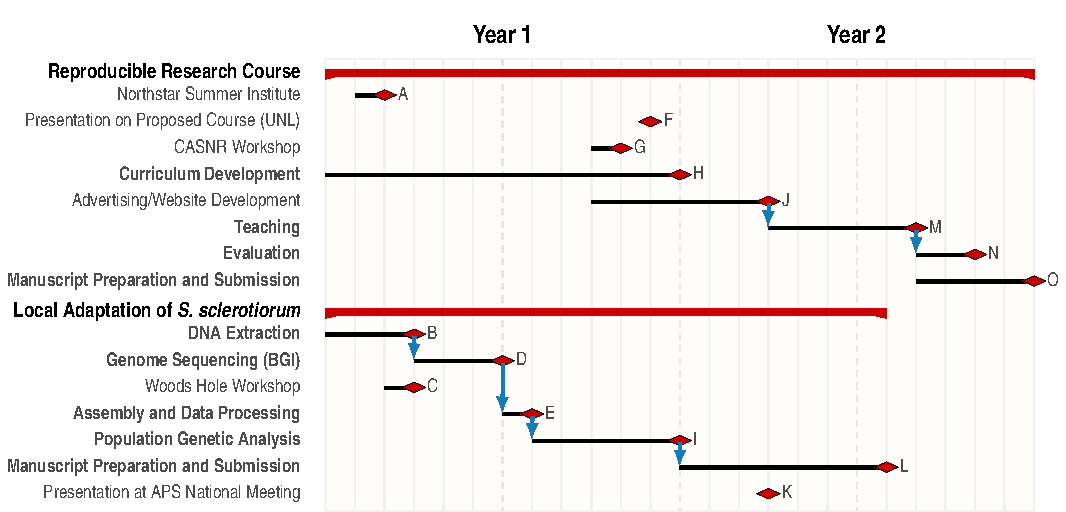
\includegraphics[width=\textwidth]{packet/timeline.pdf}
  \caption{Project Timeline. The milestones \textbf{A-N} each represent generation of a measurable outcome used in the evaluation plan.}
  \label{fig:timeline}
\end{figure}


\end{document}
